\documentclass{article}

\usepackage{graphics}
\usepackage{graphicx}
\usepackage[a4paper,
            top=2cm,
            bottom=3cm,
            left=3cm,
            right=2cm,
            marginparwidth=1.75cm
            ]{geometry}

\usepackage{float}
\usepackage{subcaption}
\usepackage{hyperref}
% \usepackage[backend=biber, style=numeric]{biblatex}

\title{TP02 - Estrutura de dados}
\author{Marcos Daniel Souza Netto - 2022069492} 
\date{\today}

\begin{document}
\maketitle

\section{Introdução}

O problema proposto consiste em implementar um programa que realiza $q$ operações de dois tipos sobre um vetor de Matrizes 2x2: O primeiro tipo consiste em uma atualização de uma posição do vetor, e o segundo tipo consiste em uma consulta sobre um intervalo do vetor (Deve ser retornado a multiplicações de todas as matrizes do intervalo e depois aplicar essa transformação linear a um vetor dado pelo usuário).

Note que uma solução ingênua para o problema seria: Dado a operação de atualização $i$ e a matriz $M$, basta atualizar a posição $i$ do vetor com a matriz $M$ (Custo constante). E para cada operação de consulta, basta percorrer o intervalo do vetor, multiplicando as matrizes e retornando o resultado e então multiplicá-lo pelo vetor. 
Porém, essa solução não é eficiente, pois uma operação de consulta desse tipo possui complexidade $O(n)$, e tendo em vista que vão ser realizadas um número grande de consultas, a complexidade passaria para $O(n \cdot q)$, onde $q$ é o número de consultas.

A solução implementada e também proposta pelos professores consiste em utilizar a ideia de \emph{Segment Tree}, que é uma estrutura de dados que permite realizar consultas em intervalos do vetor de forma eficiente. 

\section{Método}

A seguir serão detalhados a implementação da solução, de modo a explicitar 
as estruturas de dados utilizadas e as estratégias de solução. A priori vale 
apresentar as especificações do ambiente de desenvolvimento utilizado:

\begin{itemize}
    \item Sistema Operacional: Ubuntu 22.04.3 LTS;
    \item Compilador: G++ 11.4.0;
    \item Processador: Ryzen 5 5500u;
    \item Memória RAM: 8GB.
\end{itemize}


\subsection{Estruturas de dados}

Neste trabalho, foi utilizado apenas a estrutura de dados de \emph{Segment Tree}, que foi implementada no arquivo \emph{segtree.hpp}.

Como já mencionado anteriormente, essa estrutura de dados otimiza a consulta de intervalos de um vetor, e portanto, foi utilizada para otimizar a consulta de intervalos do vetor de matrizes.

A ideia é que cada nó da árvore representa um intervalo do vetor, e cada nó guarda o resultado da operação associada ao intervalo que ele representa e podemos combinar esses pedaços pré-computados para formar o resultado de uma consulta específica. Neste problema, cada nó guarda o resultado da multiplicação das matrizes do intervalo que ele representa. Assim, para realizar uma consulta, basta percorrer a árvore, e para cada nó, 
verificar se o intervalo que ele representa está contido no intervalo da consulta, caso esteja, basta retornar o valor guardado no nó, caso contrário, é necessário percorrer os filhos do nó, e repetir o processo.
Com esses pedaços, podemos combiná-los (aqui, multiplicá-los) para encontrar o resultado. Note que nessa estrutura de dados é importante que a operação a ser realizada deve ter a propriedade de associatividade (A ordem em que as operações são realizadas não altera o resultado), e no caso da multiplicação de matrizes, essa propriedade é satisfeita.

Para não entrar nos detalhes dessa estrutura de dados, a implementação utilizada foi baseada na aula 9 da Maratona UFMG, disponível em: \url{https://youtu.be/OW_nQN-UQhA?si=4qCz2jhB6BHWVRMz}. 

\subsubsection*{Propriedades da \emph{Segment Tree}} \label{sec:prop_segtree}
\begin{itemize}
    \item A altura da árvore é $O(\log n)$, onde $n$ é o número de elementos do vetor;
    \item O número total de nós da árvore é $2n -1$, onde $n$ é o número de elementos do vetor;
    \item Para a consulta de um intervalo na árvore, visitamos no máximo 4 nós por nível, temos então $O(4 \cdot \log n) = O(\log n)$, onde $n$ é o número de elementos do vetor;
\end{itemize}



\subsubsection*{Complexidade}
\begin{itemize}
    \item Para a construção da estrutura temos complexidade $O(n)$;
    \item Para a consulta na estrutura temos complexidade $O(\log n)$;
    \item Para a atualização de uma posição do vetor temos complexidade $O(\log n)$;
\end{itemize}


\subsection{Classes e principais funções}
O código foi dividido nos arquivos \emph{matrix2.hpp}, \emph{segtree.hpp} e o arquivo principal \emph{main.cpp}.
\begin{itemize}
    \item \textbf{matrix2.hpp}: Encapsulamento do tipo abstrato de dados de matriz 2x2, com as operações de multiplicação e atribuição;
        \subitem \textbf{Matrix2()}: O construtor padrão desse TAD inicializa a matriz com a matriz identidade;
        \subitem \textbf{Matrix2(int, int, int, int)}: O construtor desse TAD recebe os valores dos elementos da matriz;
        \subitem \textbf{operator*}: Sobrecarga do operador de multiplicação, que recebe uma matriz e retorna a multiplicação das duas matrizes; 

    \item \textbf{segtree.hpp}: Implementação da estrutura de dados árvore de segmentos;
        \subitem \textbf{query}: Função que recebe o intervalo da consulta e retorna a multiplicação das matrizes do intervalo;
        \subitem \textbf{update}: Função que recebe a posição do vetor a ser atualizada e a nova matriz, e atualiza a posição do vetor com a nova matriz, recalculando os valores dos nós da árvore que foram afetados pela atualização;

    \item \textbf{main.cpp}: Arquivo principal do programa que recebe os dados de entrada, os valida, e faz chamada para as funções de atualização e consulta da árvore de segmentos;
        \subitem \textbf{main}: Função principal do programa, que recebe os dados de entrada, os valida, faz chamada para as funções de atualização e consulta da árvore de segmentos e mostra o resultado das consultas na saída padrão;
    
\end{itemize}

\section{Análise de Complexidade}

A seguir serão apresentadas as análises de complexidade das principais funções do programa utilizadas na solução.
Como a parte mais importante é a implementação da árvore de segmentos, a análise de complexidade será feita para as funções de construção, consulta e atualização da árvore de segmentos.

\subsection{Construtor}
A forma implementada para a construção da árvore de segmentos foi a inicialização de todas as posições do vetor que a representa com a matriz identidade. 
Dessa forma, como o tamanho do vetor é $4n + 1$, onde $n$ é o número de transformações lineares informada na entrada, temos que a complexidade da construção da árvore é $O(n)$.

\subsection{Função \emph{query}}

Como mencionada na seção \ref{sec:prop_segtree}, a complexidade da consulta na árvore de segmentos é $O(\log n)$, onde $n$ é o número de elementos do vetor. Isso acontece porque são necessário acessar no máximo 4 nós por nível da árvore para a construção da consulta, e a altura da árvore é $O(\log n)$.

\subsection{Função \emph{update}}

De forma semelhante à função \emph{query}, para atualizar a árvore com os intervalos já pré-computados, temos que atualizar uma folha da árvore de segmentos e em seguida subir na estrutura recalculando os valores dos nós pais. 
Poranto, temos a complexidade de atualização como $O(\log n)$.

\subsection{Complexidade geral}

Analisando o programa como um todo, temos que :
\begin{enumerate}
    \item A complexidade da construção da árvore de segmentos é $O(n)$ que é realizada uma única vez;
    \item A complexidade de uma operação, tanto de consulta quanto de atualização, é $O(\log n)$, e é realizada $q$ vezes;
\end{enumerate}


Portanto, a complexidade de tempo do programa é $O(n + q \cdot \log n)$, onde $n$ é o número de transformações lineares informada na entrada e $q$ é o número de consultas informada na entrada.
Já a complexidade de espaço é $O(n)$, pois é necessário armazenar a árvore de segmentos, que neste caso tem o tamanho de $4n + 1$.

\section{Estratégias de robustez}
Com a utilização da biblioteca \emph{msgassert}, presente no arquivo \emph{msgassert.h}, foi implementada a verificação do domínio dos dados de entrada, especificados na descrição do trabalho. 
Quando o dado de entrada não respeita o domínio especificado, o programa é encerrado e uma mensagem do erro específico é exibida na saída padrão de erro.

\section{Análise Experimental}

A seguir serão apresentados os resultados obtidos na experimentação do programa.

\subsection{Localidade de Referência}

Utilizando o programa \emph{analisamem}, fornecido pelos professores, foi possível observar a localidade de referência do programa. 
Para isso, foi utilizado o programa de geração de casos de testes, também fornecido pelos professores, para gerar uma entrada que realiza 1000 operações (consulta e atualização) em um vetor de 1000 posições.

Além disso, é importante salientar que toda a análise de localidade será feita sobre a estrutura principal do trabalho, a árvore de segmentos.

\begin{figure}[H]
    \centering
    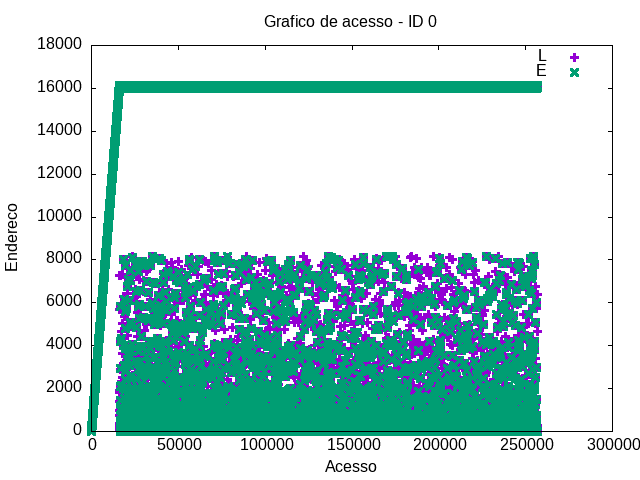
\includegraphics[width=0.6\textwidth]{./images/registro-acesso-0.png}
    \caption{Leitura e escrita na memória}
    \label{fig:ac01}
\end{figure}

Essa figura é bastante interessante e informativa, pois mostra por meios práticos o funcionamento de uma árvore de segmentos: 
Note que a base do "retângulo" da figura é mais preenchida do que sua parte superior, isso se deve porque os nós mais próximos da raiz, na implementação utilizada, estão em endereços mais baixos enquanto as folhas estão em endereços mais altos. 
\begin{itemize}
    \item Em consultas, o intuito de se utilizar árvore de segmentos é exatamente utilizar de cálculos já precomputados e assim acessar menos os valores orginais do próprio vetor. Desse modo, utiliza-se dos valores que estão em endereços mais baixos no gráfico. Eventualmente, caso necessário, a estrutura deve descer para posições próximas das folhas, mas como mostrado no gráfico, ocorre com menos frequência.
    \item Em atualizações, o comportamento é semelhante ao anterior, com a diferença que obrigatoriamente é necessário descer para as folhas e assim recalculando os nós que estão no caminho da folha atualizada até a raiz. É fácil ver que também temos acessos mais frequentes para nós próximos da raiz afinal esse é o comportamento da própria operação de atualização.
\end{itemize}

\begin{figure}[H]
    \centering
    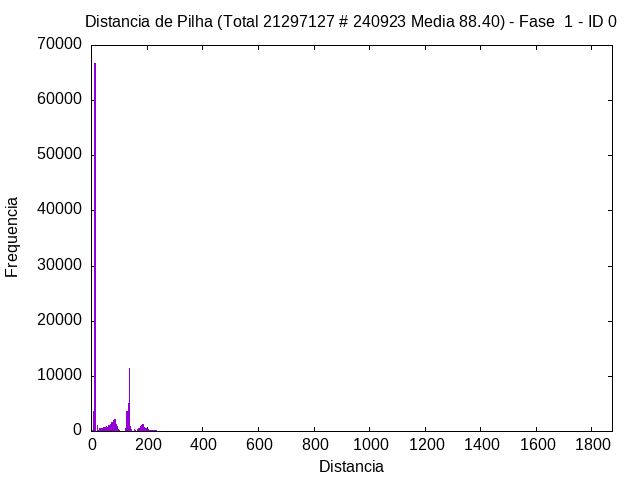
\includegraphics[width=0.6\textwidth]{./images/registro-hist-1-0.png}
    \caption{Distâcia de Pilha}
    \label{fig:ac02}
\end{figure}

A figura acima reafirma o argumento anterior: Alguns nós são acessados muito mais vezes do que outros. Isto é, nós mais proximos da raiz, devido o próprio comportamento da árvore de segmentos, são acessados com maior frequência.


\begin{figure}[H]
    \centering
    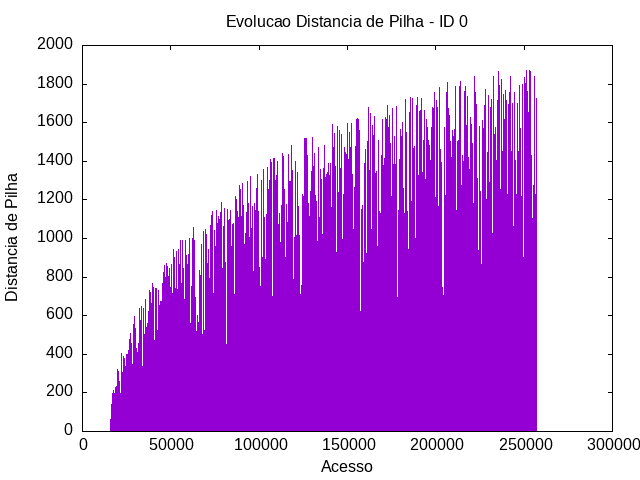
\includegraphics[width=0.6\textwidth]{./images/registro-distp-0.png}
    \caption{Evolução de Distância de Pilha}
    \label{fig:ac03}
\end{figure}

% A figura \ref*{fig:ac03} mostra a evolução da pilha ao passar da execução do programa.


\section{Conclusões}

O trabalho proposto foi de grande valia para o aprendizado de estruturas de dados, e de como elas podem ser utilizadas para resolver de forma muito mais eficientes certos problemas. Neste caso, a estrutura de árvore de segmentos provê de forma eficiente operações de atualização e consulta sobre um vetor cuja operações sobre o dado tem propriedade associativa.

\section*{Bibliografia}

\begin{itemize}
    \item Slides da disciplina de Estrutura de Dados, ministrada pelo Prof. Wagner Meira Jr. e Prof. Eder Fereira Figuiredo.
    \item Aula 9 - SegTree, Maratona UFMG. 
    \subitem Disponível em: \url{https://youtu.be/OW_nQN-UQhA?si=4qCz2jhB6BHWVRMz}
    
\end{itemize}


\section*{Instruções para compilação e execução}

É necessário ter instalado na máquina o compilador g++, com pelo mínimo a versão descrita no começo do trabalho.  

Em um terminal, navegue até a pasta raiz do projeto e execute os seguintes comandos:

\begin{verbatim}
    $ make
    $ ./tp03.out

\end{verbatim}

Agora, basta seguir o padrão de entrada descrito na especificação do trabalho.


\end{document}